\section{Introduction}

In this paper we describe \OurSys, an in-network distributed mitigation for
faulty links.  We claim that our design requires minimal configuration, is
transparent to end-points~\cite{Saltzer84end-to-endarguments} and does not
conflict with existing network architecture choices (e.g., what topology to use
and how to route over it). We model \OurSys using ns-3 and evaluate
implementations for CPUs and FPGAs.

\paragraph{Contributions.}
\amd{What are we claiming as contributions? (not clear to me...and we need
  to make it crystal clear to potential reviewers) (1) proposal-of/strategy-for using FEC for wired
  links in dater center? (2) link adaptation scheme? (3) 10Gbps FPGA implementation?}

The next section describes the background and related work of the problem we
are solving, before we describe our design~(\S\ref{sec:design}) and
implementation~(\S\ref{sec:implementation}), which we
evaluate~(\S\ref{sec:evaluation}) before concluding.

\begin{figure}
  \centering
  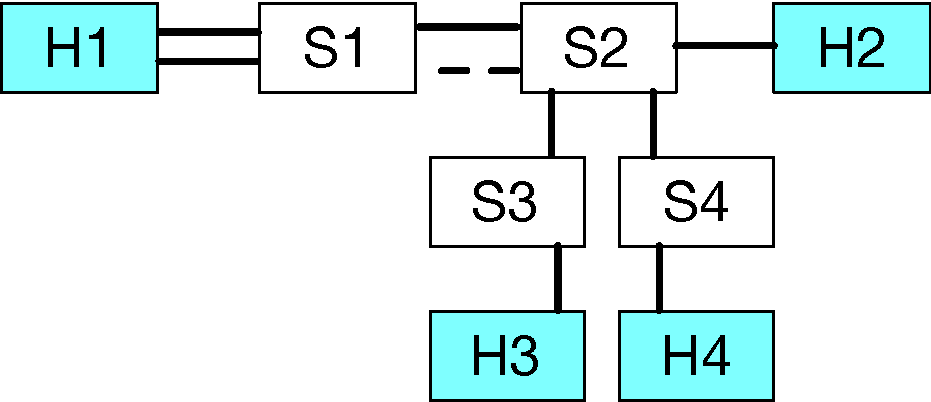
\includegraphics[width=0.3\paperwidth]{example_network.pdf}
  \caption{\label{fig:example-net}An example network consisting of four
    switches (S1-S4) and four hosts (H1-H4). Faulty links are shown as dashed lines.
    Each link is assumed to have capacity $R$ unless the link is faulty, in
    which case it has capacity $F < R$.  In this example, the failing link
    diminishes the bandwidth of H1.}
\end{figure}
